\documentclass{article}
\usepackage[utf8x]{inputenc}
\usepackage[russianb]{babel}
\usepackage[usenames]{color}
\usepackage{vmargin}
\usepackage{ amssymb }
\usepackage{listings}
\usepackage[linesnumbered,boxed]{algorithm2e}
\usepackage{graphicx}
\usepackage{amsthm}
\usepackage{setspace}
\usepackage{indentfirst}
\usepackage[noend]{algorithmic}
\onehalfspacing
\setpapersize{A4}
\setmarginsrb{3cm}{2cm}{3cm}{2cm}{0pt}{0mm}{0pt}{13mm}
\sloppy
\renewcommand\contentsname{Оглавление}
\renewcommand{\labelenumi}{\theenumi)}

\begin{document}

\null\hfill\begin{tabular}[t]{l@{}}
	\textit{Kirill Zuev}
\end{tabular}

\begin{center}
	\textbf{Home assignment № 3}
\end{center}

\textbf{Task 2.}

The minimal subset of implications from which all of given are deducible is:
$$
\{ A \to C,\ C \to E,\ E \to B,\ E \to D,\ DB \to C \}
$$

For getting $C \to D$ use 3-rd axiom: $\{ C \to E,\ E \to D \} \Rightarrow C \to D$.\\

For getting $BC \to D$ use 2-nd axiom: $C \to D \Rightarrow BC \to D$.\\

For getting $A \to E$ use 3-rd axiom: $\{ A \to C,\ C \to E \} \Rightarrow A \to E$.\\

For getting $AB \to D$ use 2-nd and 3-rd axioms.

3-rd axiom: $\{ A \to E,\ E \to D \} \Rightarrow A \to D$;

2-nd axiom: $A \to D \Rightarrow AB \to D$.\\

If we remove any implication from our minimal subset then we couldn't get all needed implications.
\clearpage

\textbf{Task 4.}

\begin{figure}[h!]
	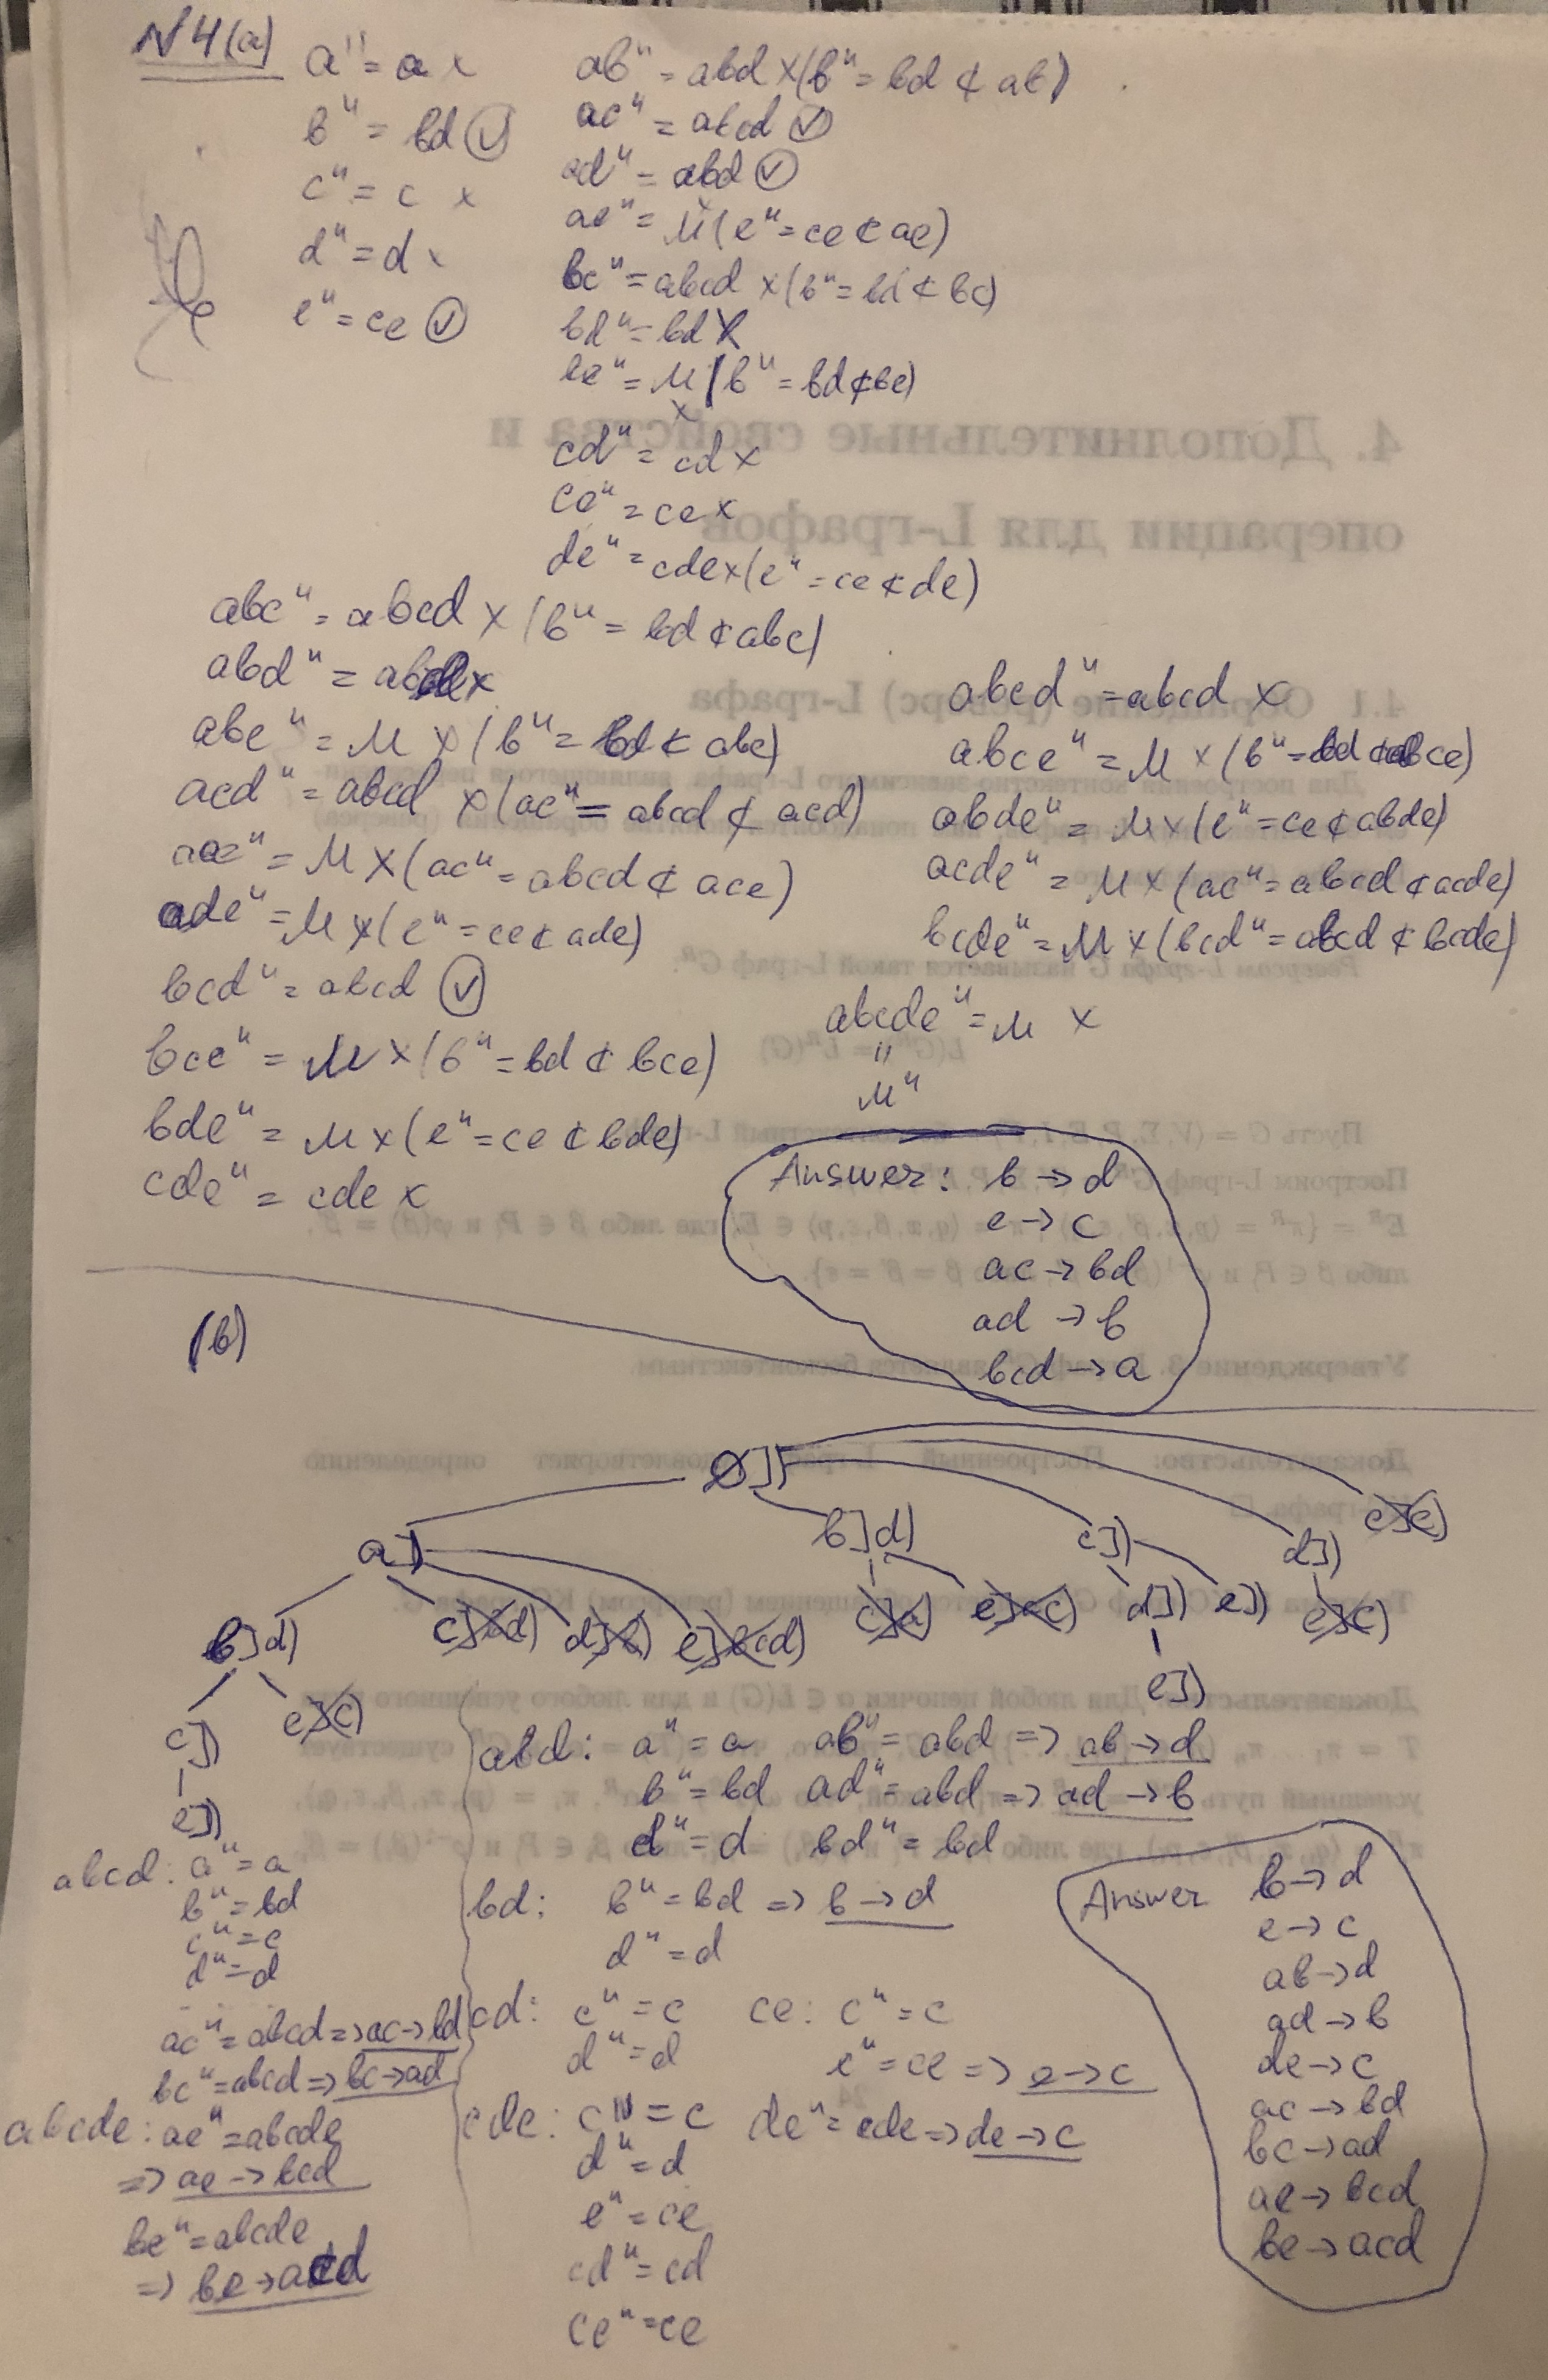
\includegraphics[width=15cm]{4.jpg}
\end{figure}

 \end{document}